%%%%%%%%%%%%%%%%%%%%%%%%%%%%%%%%%%%%%%%%%%%%%%%%%%%%%%%%%%%%%%%%%
%2345678901234567890123456789012345678901234567890123456789012345
%        1         2         3         4         5         6     
\chapter{Experimental result}
\label{cha:experiment}
 The experiment is conducted both in simulation and ABB test prototype through collecting sensor feedback and apply forward kinematic on it.
The main design objective of our controller is it's performance under inconsistent task space command.

In this chapter we test 3 trajectories each represent a typical situation. 
\begin{itemize}
    \item[1] Pure rotation trajectory. From initial position, the platform makes a 360 degree rotation while the $\dot{x},\dot{y}$ remains 0 all the time.
    \item[2] 90 degree turn of heading. The task space velocity change from $\dot{\xi}=[1,0,0]$ to $\dot{\xi}=[0,1,0]$ in one control cycle.
    \item[3] Translation with rotation. Move 10 meters along x direction and rotate 360 degree simultaneously
\end{itemize}
The pure rotation trajectory require a sudden change of ICR position from infinite far away to origin, which corresponding to a 45 degree sudden change on steering angles. This most part of this trajectory will trigger the ICR control logic so it is used to test the ICR controller performance.

The 90 degree turn trajectory does not involve and angular velocity so the ICR is always infinite far away, thus only approximation based inverse kinematic control logic will be triggered. Thus this trajectory is used to test the performance of IKAM control logic.

The translation with rotation trajectory represents the general cases, where the task space command is generally smooth and ICR is changing position so that switching between 2 control logics happens frequently. Thus this trajectory is to test the general performance and the switching.
\begin{table}[!ht]
	\centering
		\begin{tabular}{cc}
		Trajectories   &  control strategy triggered                  \\\midrule
		Pure rotation          &  ICR, IKAM     \\
		90 degree turn          &  IKAM              \\
		Translation with rotation      &  ICR, IKAM              \\\bottomrule
		\end{tabular}
		\vspace{1mm}
	\caption{Nomenclature of the MPC approaches}
	\label{tab:testTrajectory}
\end{table}
This chapter is then divided by 4 sections, 3 of them explain 3 test trajectory and the last section discuss the advantage and problem we observe in the experiment.
%%%%%%%%%%%%%%%%%%%%%%%%%%%%%%%%%%%%%%%%%%%%%%%%%%%%%%%%%%%%%%%%%%%%%%%%%%%%%%%%%%%%%%%%%%%%%%%%%%%%%%%%
%%%%%%%%%%%%%%%%%%%%%%%%%%%%%%%%%%%%%%%%%%%%%%%%%%%%%%%%%%%%%%%%%%%%%%%%%%%%%%%%%%%%%%%%%%%%%%%%%%%%%%%%
\section{Pure rotation trajectory}
\label{sec:pureRotationTraj}
\subsection{Task space velocity performance}
For this trajectory, the reference command has no translation velocity, which means $\dot{x}_{ref}=0, \dot{y}_{ref}=0$ holds all the time. While the $\dot{\theta}_{ref}$ is a function of time which is illustrate in \cref{fig:PR_t} as reference signal. The controller generated response $\dot{x}_{hat}$ is also shown in the figure, and we can see that it takes around 1 second for the platform to do the initialization, and after that the wheel is oriented to the desired position, and the reference command is perfectly followed.
\begin{figure}[!h]
    \centering
    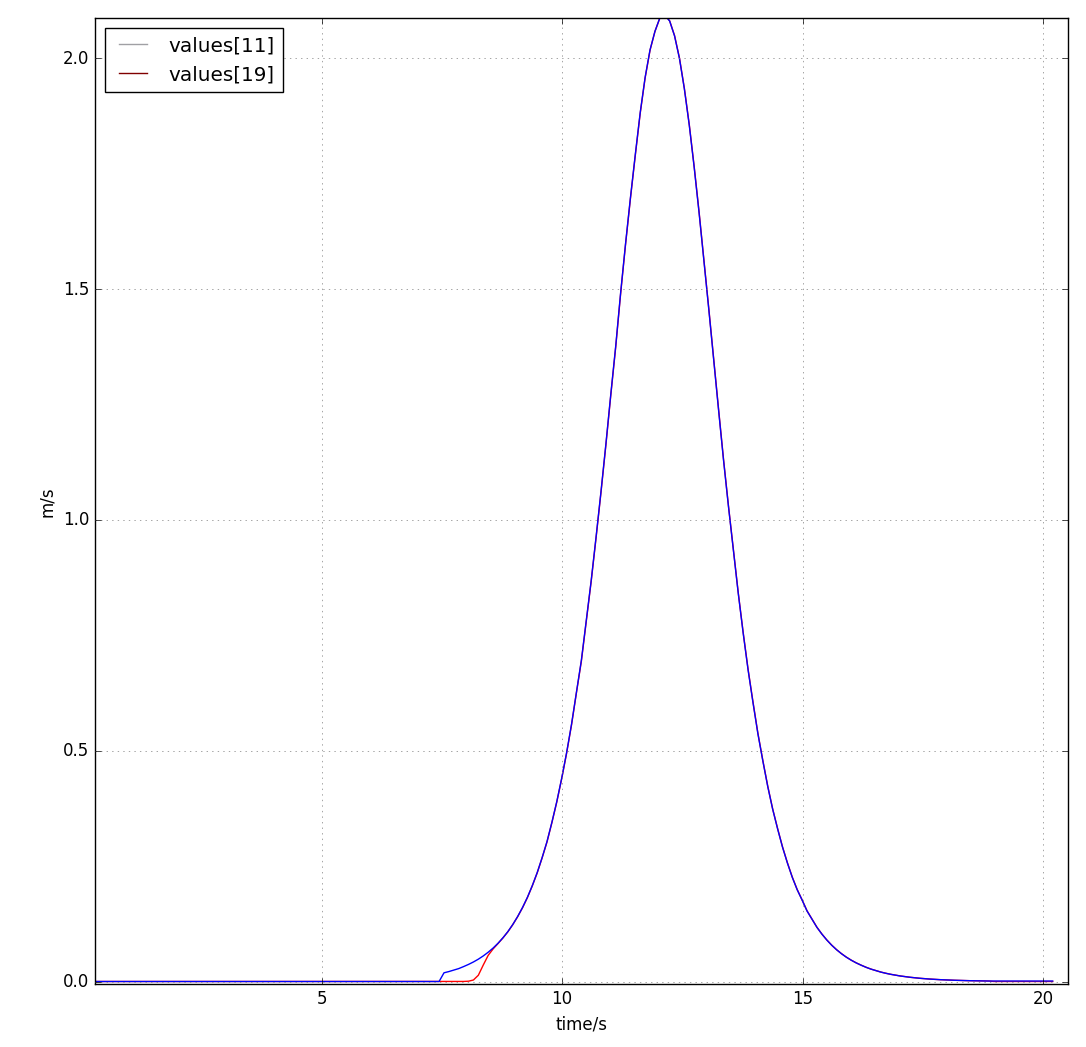
\includegraphics[width=0.6\textwidth]{Figures/PR_t.png}  
    \caption{Reference command and response on $\dot{\theta}$}
    \label{fig:PR_t}
\end{figure}

Then we look into the $\dot{x}$ and $\dot{y}$ performance in \cref{fig:PRtranslation}, we can see that even though the reference command remains 0 for both direction, the generated response still have a small velocity on $\dot{x}$ direction in \cref{fig:PRtranslationX}. That is due to the fact that the initial wheel orientation cannot conduct pure rotation command, this is constrained by the DoM. And the intermediate $\Tilde{\dot{\xi}}_{ref}$ generated by ICR control logic will contain a small component on x direction to make $\Tilde{\dot{\xi}}_{ref}$ respect kinematic constraint. The small disturbance between $t=10-20s$ is caused by accuracy issue of optimization algorithm.
\begin{figure}[!hb]
     \centering
     \begin{subfigure}[b]{0.49\textwidth}
         \centering
          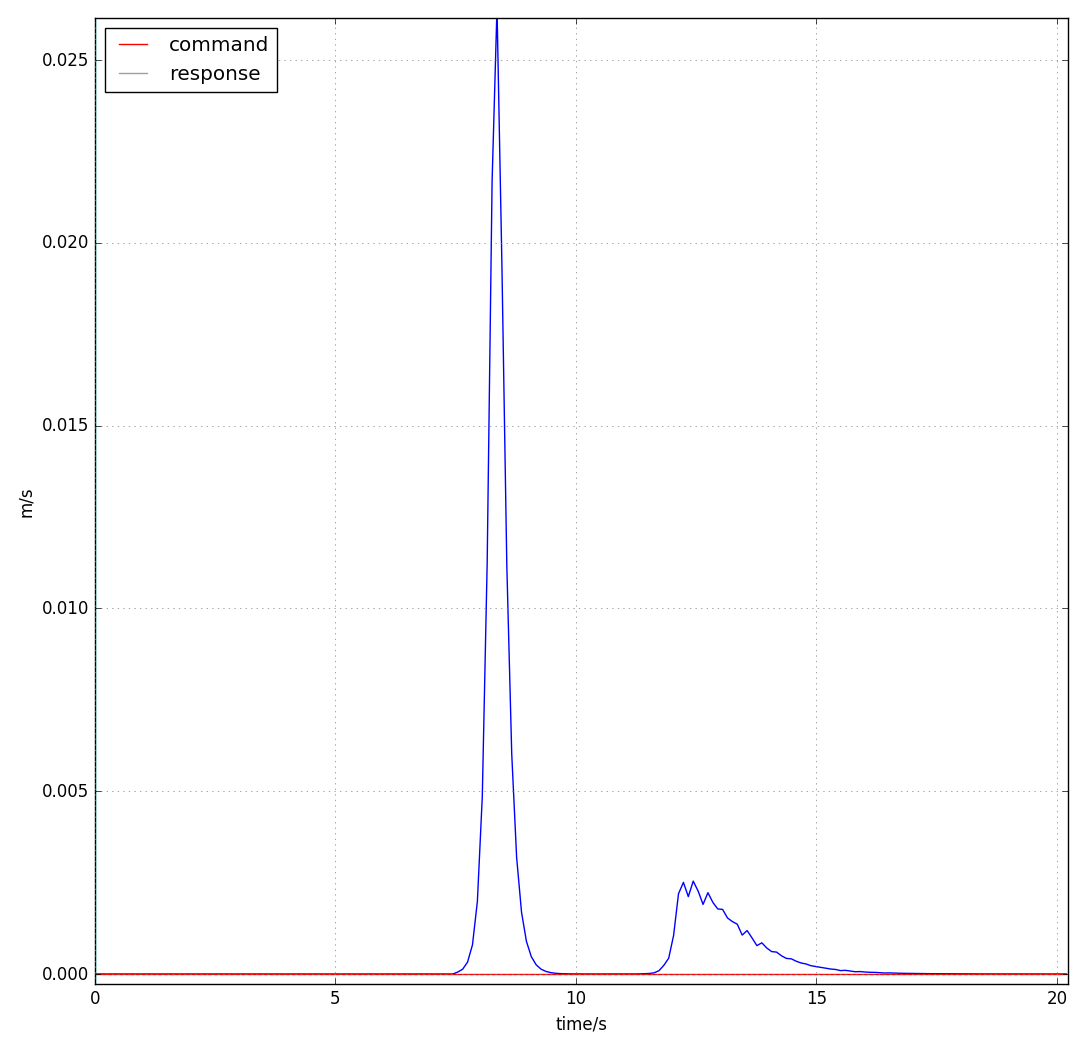
\includegraphics[width=1.2\textwidth]{Figures/PR_x.png}
         \caption{$\dot{x}$}
         \label{fig:PRtranslationX}
     \end{subfigure}
     \hfill
     \begin{subfigure}[b]{0.49\textwidth}
         \centering
         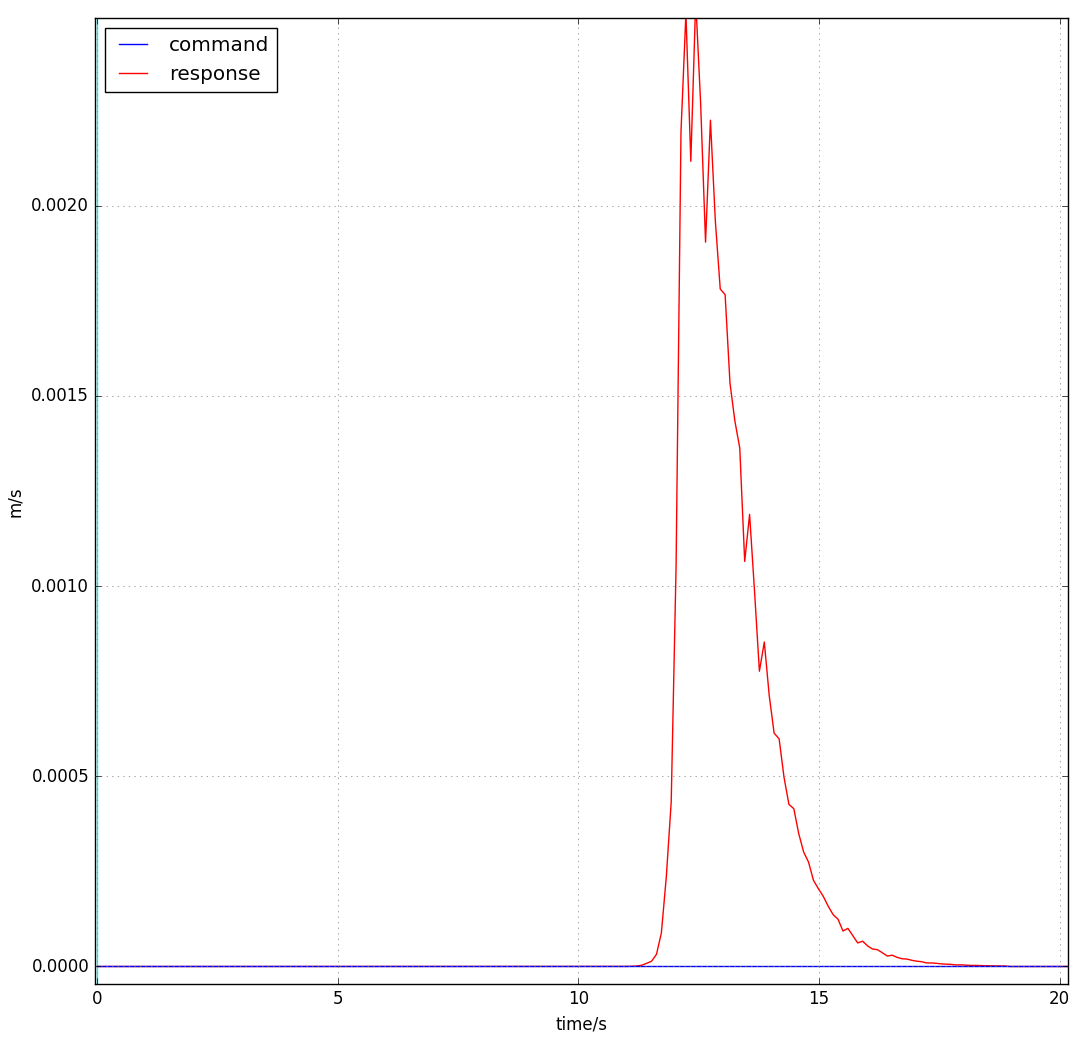
\includegraphics[width=1.2\textwidth]{Figures/PR_y.png}
         \caption{$\dot{y}$}
         \label{fig:PRtranslationY}
     \end{subfigure}
     
        \caption{translation velocity}
        \label{fig:PRtranslation}
\end{figure}
%%%%%%%%%%%%%%%%%%%%%%%%%%%%%%%%%%%%%%%%%%%%%%%%%%%%%%%%%%%%%%%%%%%%%%%%%%%%%%%%%%%%%%%%%%%%%%%%%%%%%%%%
\subsection{ICR response}
Our controller directly manipulate on ICR, so the output $ICR_{next}$ contain a lot of information of the controller behavior. As shown in \cref{fig:PR_ICRx}, the x component of reference ICR keeps 0 along the trajectory, but due to constraint and optimization accuracy issue, the executed $ICR_{next}$ is slightly deviated from 0. And if we look at \cref{fig:PR_ICRy}, the y component of $ICR_{ref}$ also keeps 0 along the trajectory. The control logic switch to ICR control at time $t=3.5$ and the response y component of $ICR_{next}$ start from a very large value, and smoothly move to the desired value. The whole process takes less than 1 second.
\begin{figure}[!h]
    \centering
    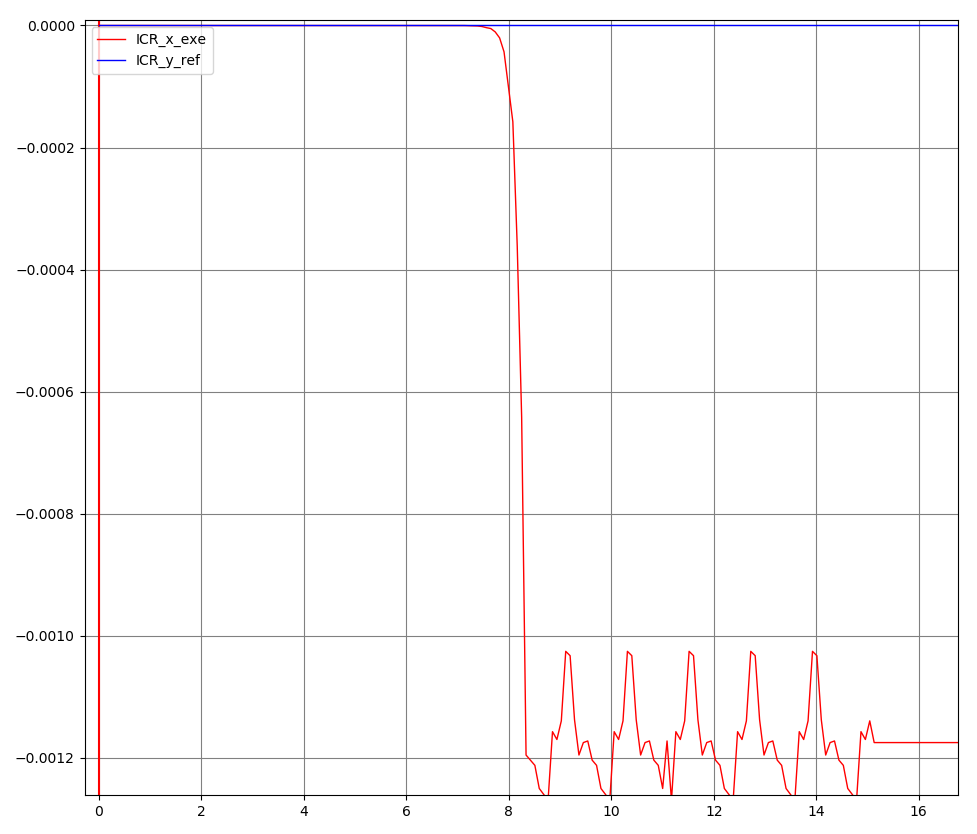
\includegraphics[width=\textwidth]{Figures/PR_ICR_x.png}
    \caption{$\Tilde{ICR_x}$ }
    \label{fig:PR_ICRx}
\end{figure}

\begin{figure}[!h]
    \centering
    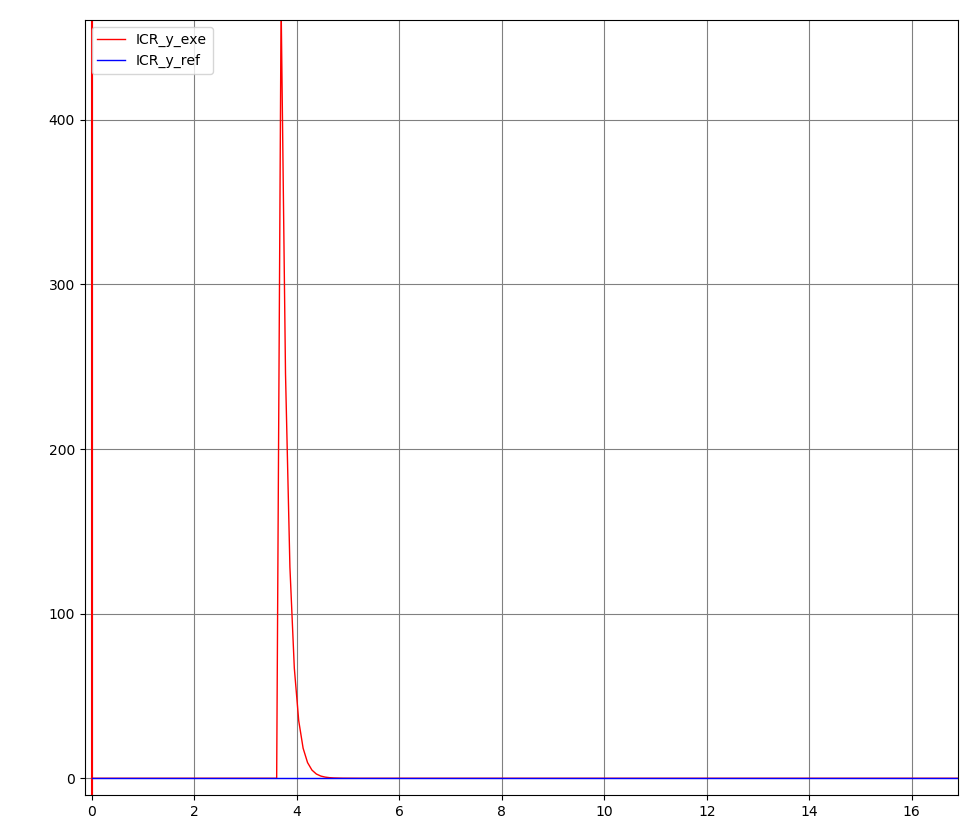
\includegraphics[width=1\textwidth]{Figures/PR_ICR_y.png}
    \caption{$\Tilde{ICR_y}$ }
    \label{fig:PR_ICRy}
\end{figure}
%%%%%%%%%%%%%%%%%%%%%%%%%%%%%%%%%%%%%%%%%%%%%%%%%%%%%%%%%%%%%%%%%%%%%%%%%%%%%%%%%%%%%%%%%%%%%%%%%%%%%%%%
%%%%%%%%%%%%%%%%%%%%%%%%%%%%%%%%%%%%%%%%%%%%%%%%%%%%%%%%%%%%%%%%%%%%%%%%%%%%%%%%%%%%%%%%%%%%%%%%%%%%%%%%
\section{Turning 90 degree}
\label{sec:90degree}
Through out this trajectory, $\dot{\xi}_{ref}$ changes from $[1,0,0]$ to $[0,1,0]$ and end up with $[-1,0,0]$. Appears to be 90 degree turning of heading for 2 times. While the $\dot{\theta}$ component of $\dot{\xi}_{ref}$ keeps being 0, which means no rotation involved in the trajectory.

The ICR keeps being infinite far away through out the trajectory, the ICR control logic will not be triggered. And the Approximation based control logic is examined. The performance on x and y direction is shown in \cref{fig:90}. The trajectory has 3 inconsistency points, at time $t=4$ the reference signal changes from $\dot{\xi}=[0,0,0]$ to $\dot{\xi}=[1,0,0]$, no steering angle change is needed here as $\dot{\xi}=[1,0,0]$ require the same steering angle as the initial state. So that we can see the response of wheel almost perfectly match the reference.

At $t=8$ reference changes to $\dot{\xi}=[0,1,0]$, here a 90 degree sudden change of steering angle is needed and we can see that the it takes around 1 second for the intermediate reference $\dot{\xi}$ to reach the target.

And at $t=12.2$ the reference end up with $\dot{\xi}=[-1,0,0]$. the behavior is similar as before.  The reference signal in the figure is what we used to give motor command, but the motor control it self is not with in our scope. One thing to be noticed is that the steer motors have slight overshot for this trajectory.
\begin{figure}[!hb]
     \centering
     \begin{subfigure}[b]{0.49\textwidth}
         \centering
          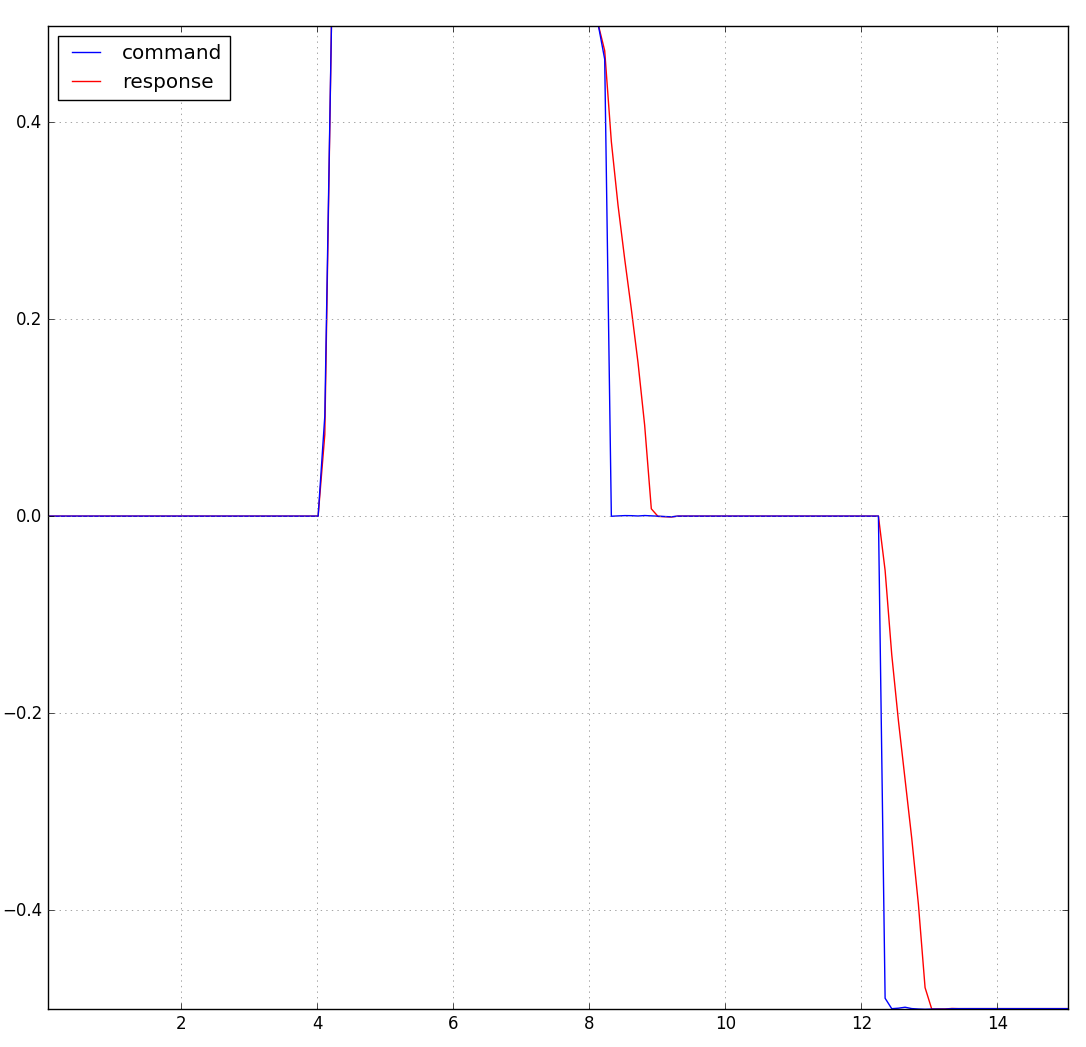
\includegraphics[width=1.1\textwidth]{Figures/90_x.png}
         \caption{$\dot{x}$}
         \label{fig:90X}
     \end{subfigure}
     \hfill
     \begin{subfigure}[b]{0.49\textwidth}
         \centering
         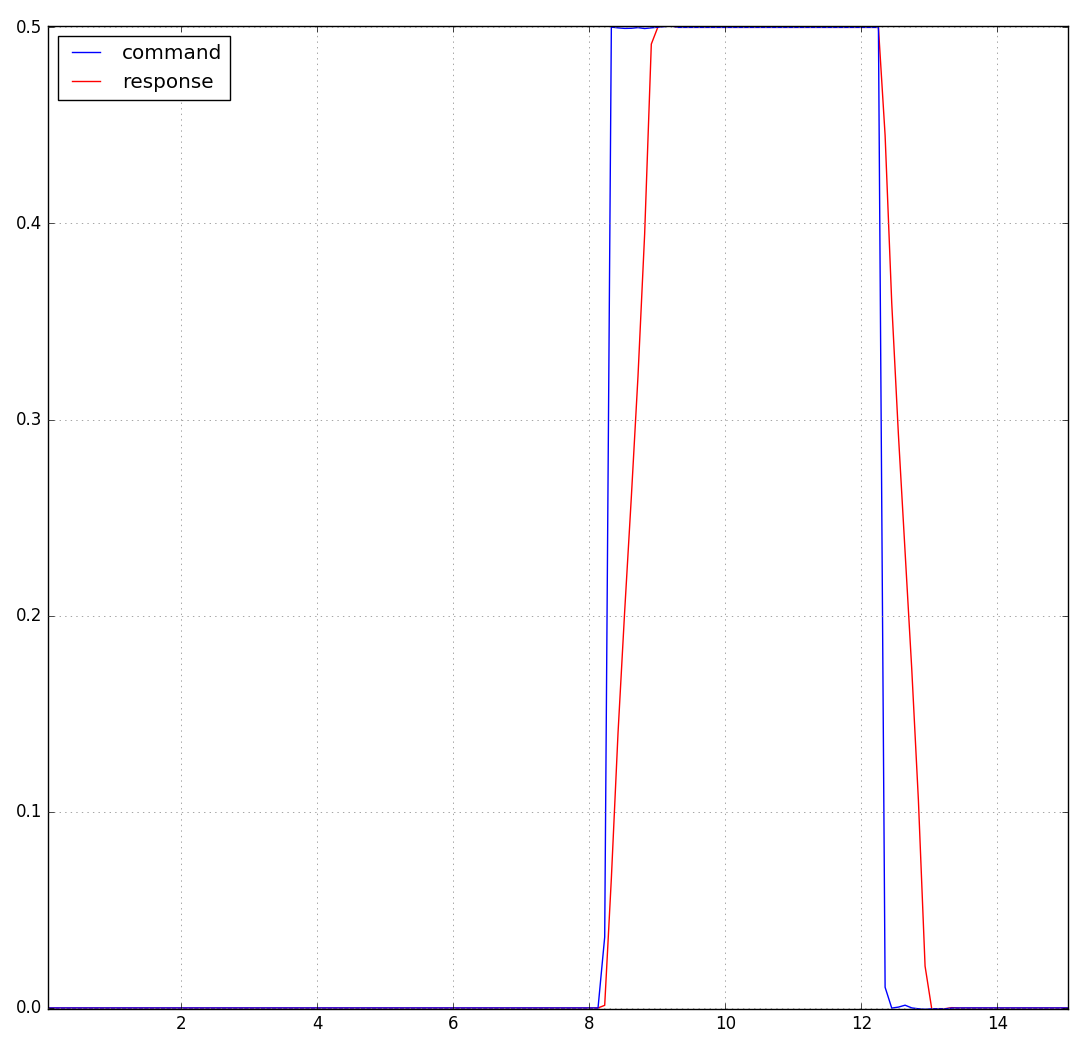
\includegraphics[width=1.1\textwidth]{Figures/90_y.png}
         \caption{$\dot{y}$}
         \label{fig:90Y}
     \end{subfigure}
     
        \caption{translation velocity}
        \label{fig:90}
\end{figure}
% \begin{figure}[!ht]
%     \centering
%     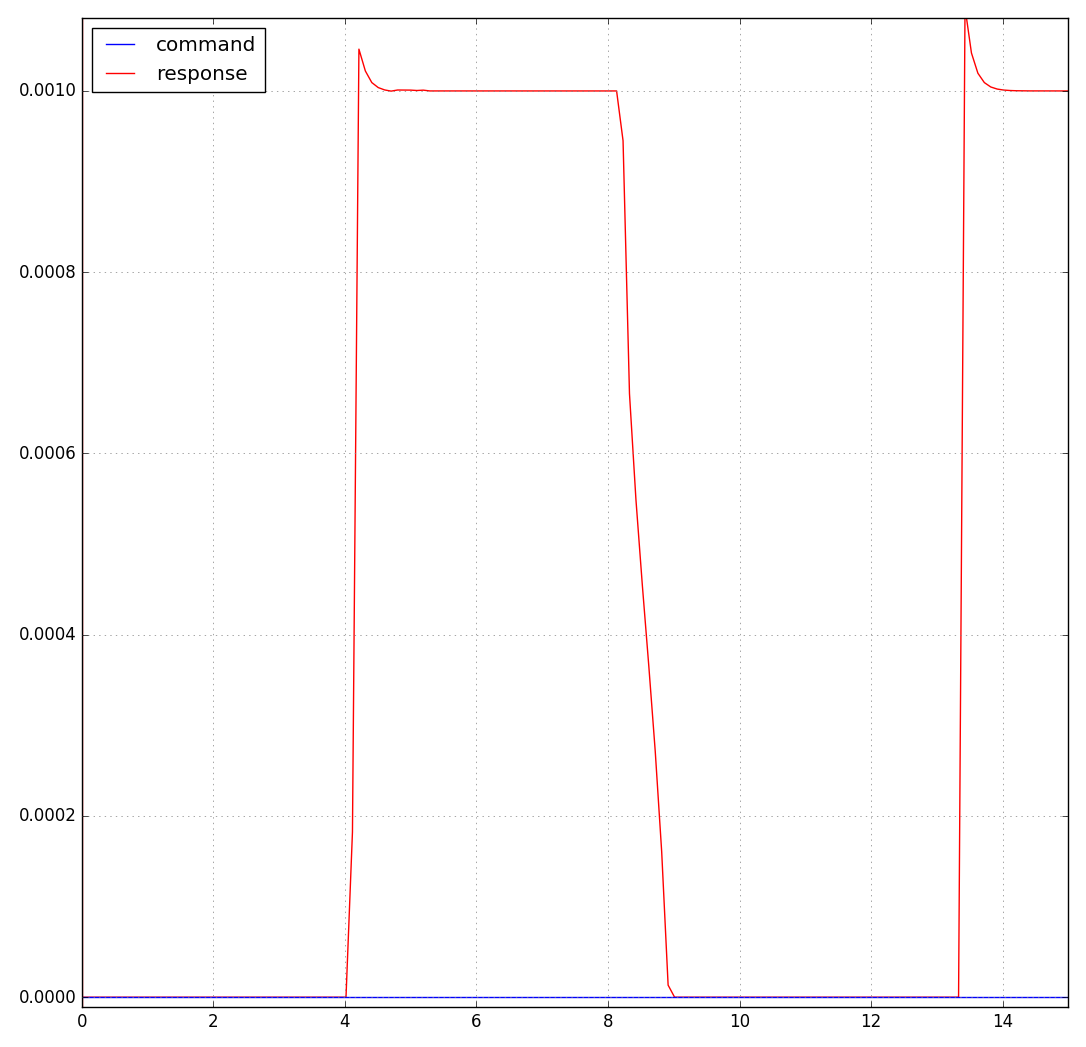
\includegraphics[width=0.7\textwidth]{Figures/90_t.png}
%     \caption{Caption}
%     \label{fig:my_label}
% \end{figure}

% \begin{figure}[!h]
%     \centering
%     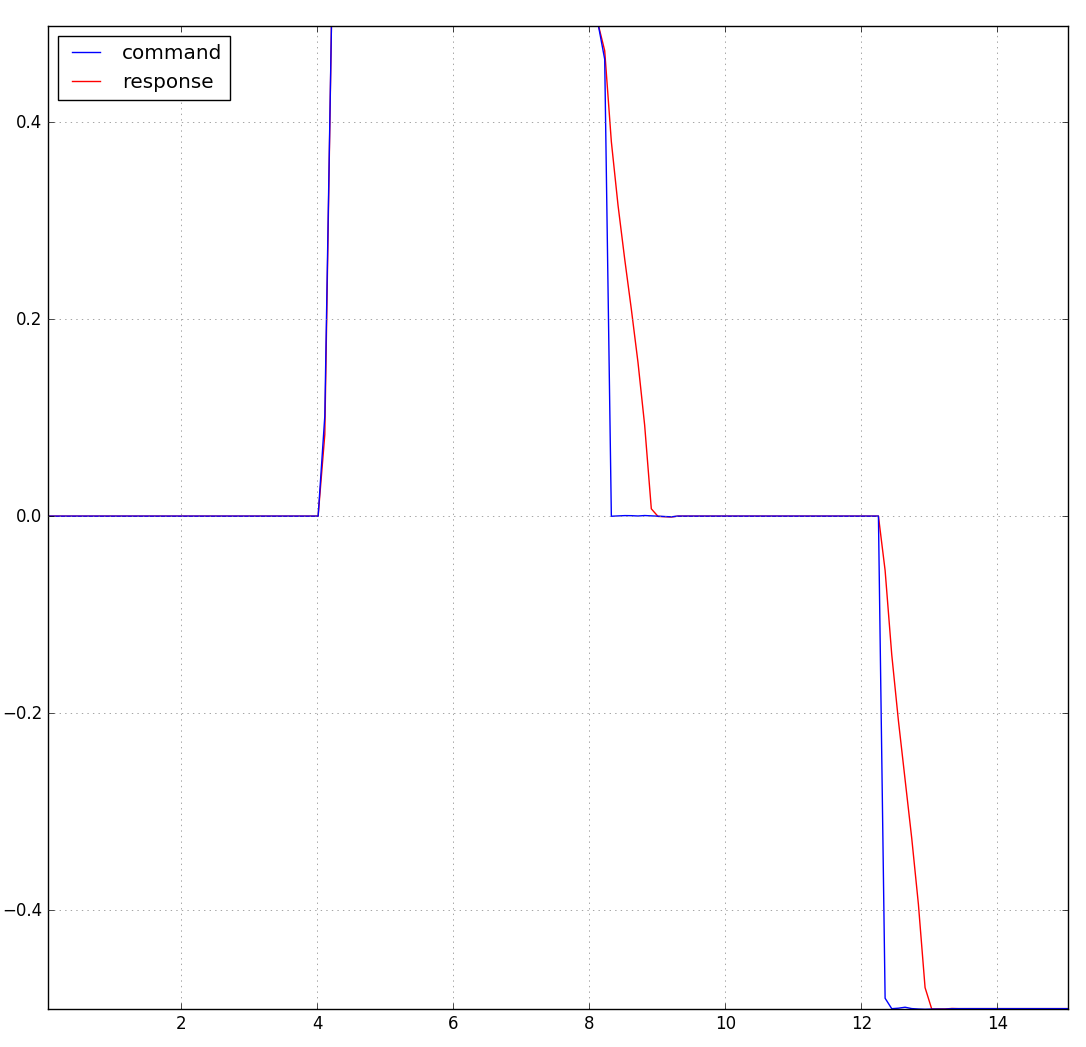
\includegraphics[width=0.7\textwidth]{Figures/90_x.png}
%     \caption{Caption}
%     \label{fig:my_label}
% \end{figure}
% \begin{figure}[!h]
%     \centering
%     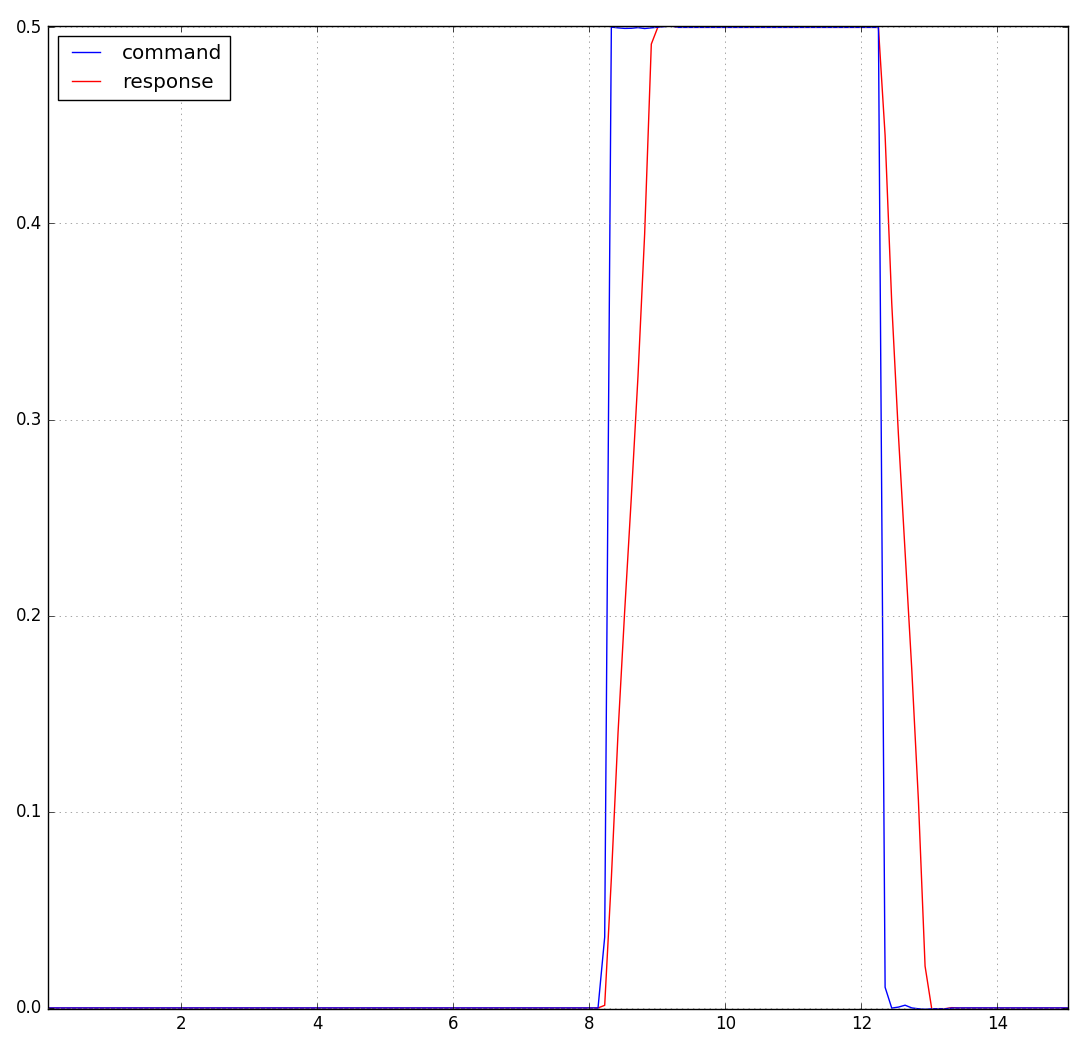
\includegraphics[width=0.7\textwidth]{Figures/90_y.png}
%     \caption{Caption}
%     \label{fig:my_label}
% \end{figure}


%%%%%%%%%%%%%%%%%%%%%%%%%%%%%%%%%%%%%%%%%%%%%%%%%%%%%%%%%%%%%%%%%%%%%%%%%%%%%%%%%%%%%%%%%%%%%%%%%%%%%%%%
%%%%%%%%%%%%%%%%%%%%%%%%%%%%%%%%%%%%%%%%%%%%%%%%%%%%%%%%%%%%%%%%%%%%%%%%%%%%%%%%%%%%%%%%%%%%%%%%%%%%%%%%
\section{Translation with rotation}
For this trajectory, the platform is moving along x direction with constant velocity, and rotate for 360 degree at the same time with the angular velocity as a function of time $\dot{\theta}=\frac{1}{1+exp(t-t_d)}$, where $t_d=5s$ is a delay factor. For this trajectory the ICR is moving around with a relative high velocity and switching between 2 control logic happens twice.

\subsection{Task space velocity response}
The response on the task space velocity have small error in this case, this is due to the fact that the changing of $\dot{\xi}$ result in fast change of joint response $\dot{\beta}, \dot{\phi}$ and thus been damped. This could be a big drawback if the robot is conducting accuracy-critical missions, in this case the platform might not conduct the exact incoming command.
\begin{figure}[H]
    \centering
    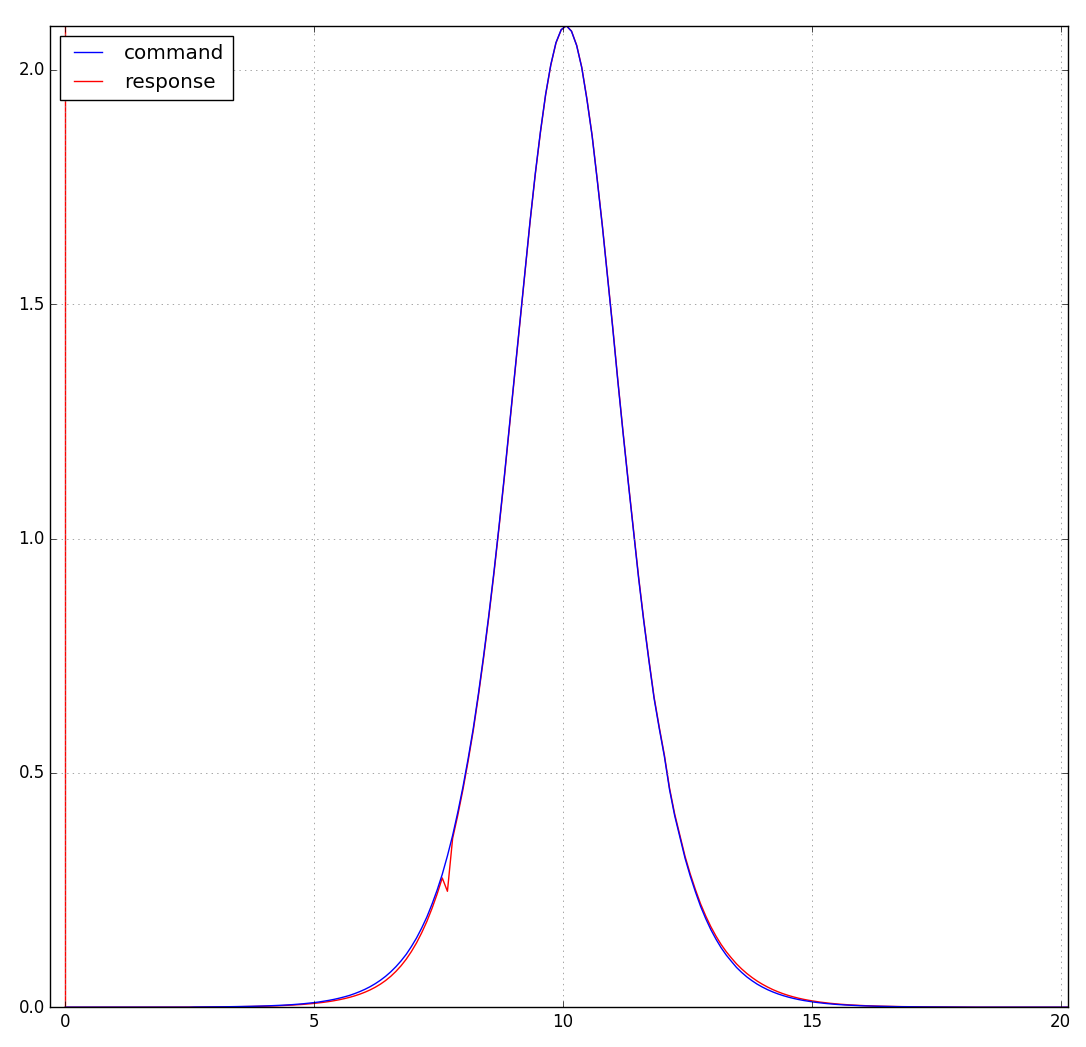
\includegraphics[width=\textwidth]{Figures/360_t.png}
    \caption{Angular velocity $\dot{\theta}$}
    \label{fig:my_label}
\end{figure}

\begin{figure}[H]
     \centering
     \begin{subfigure}[b]{0.49\textwidth}
         \centering
          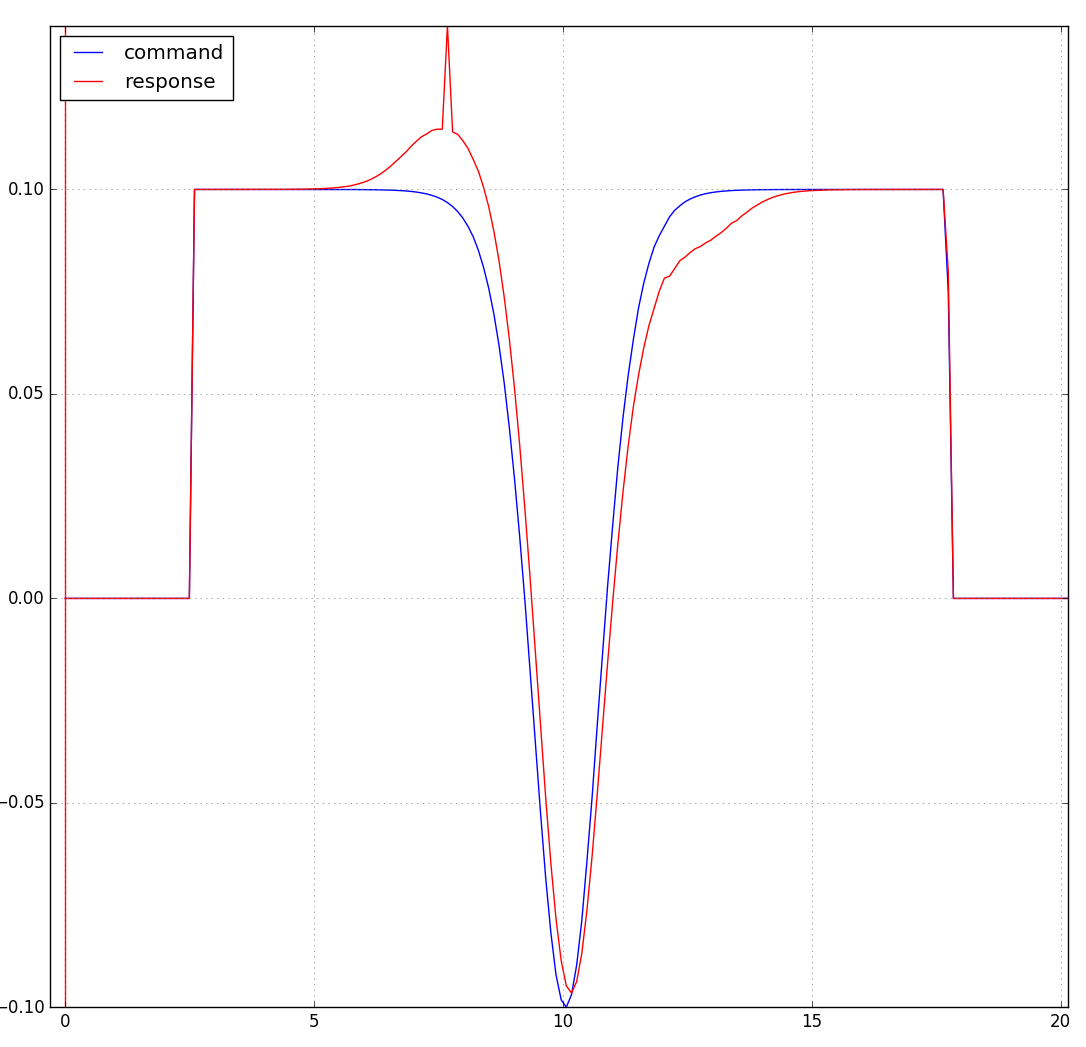
\includegraphics[width=1.05\textwidth]{Figures/360_x.png}
         \caption{$\dot{x}$}
         \label{fig:360X}
     \end{subfigure}
     \hfill
     \begin{subfigure}[b]{0.49\textwidth}
         \centering
         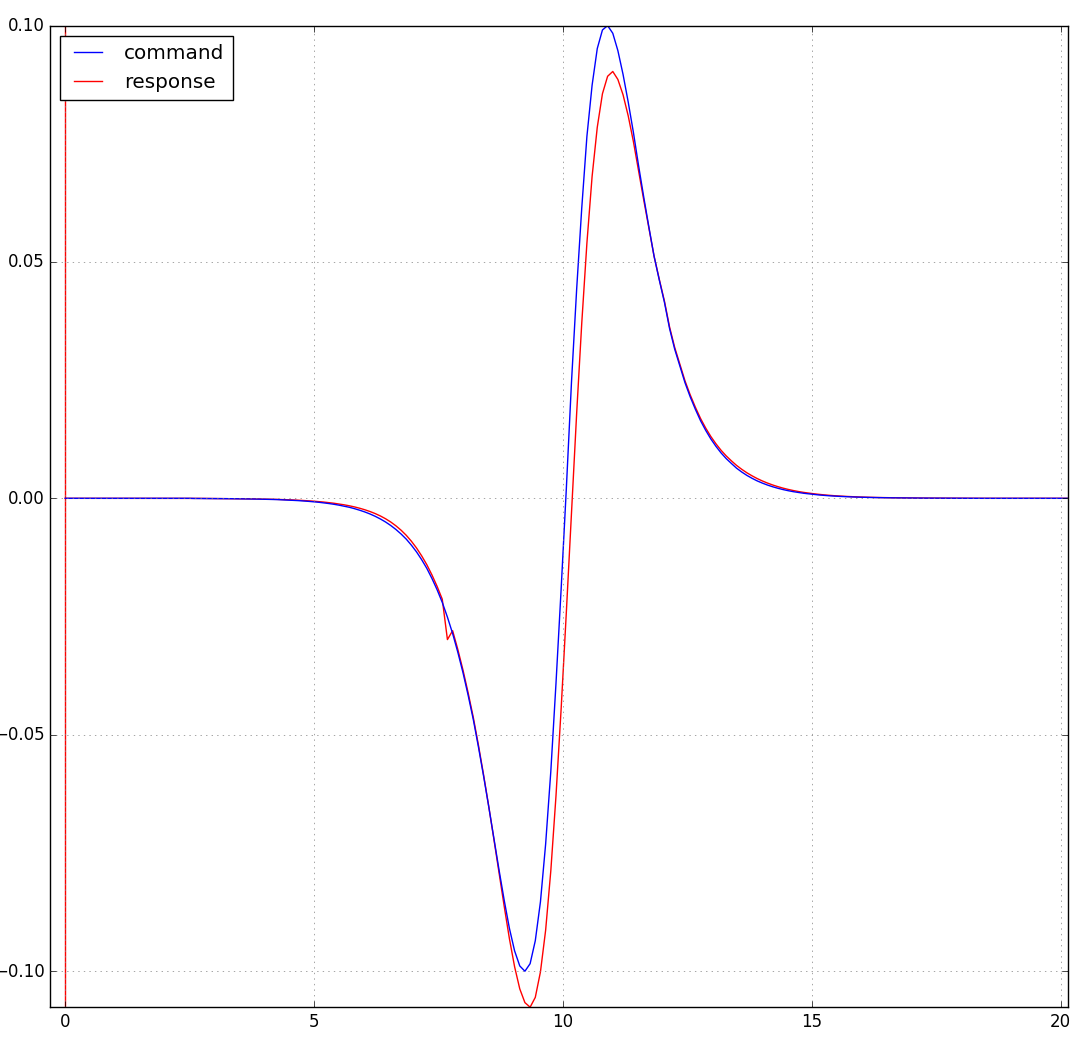
\includegraphics[width=1.05\textwidth]{Figures/360_y.png}
         \caption{$\dot{y}$}
         \label{fig:90Y}
     \end{subfigure}
     
        \caption{translation velocity}
        \label{fig:360}
\end{figure}
% \begin{figure}[H]
%     \centering
%     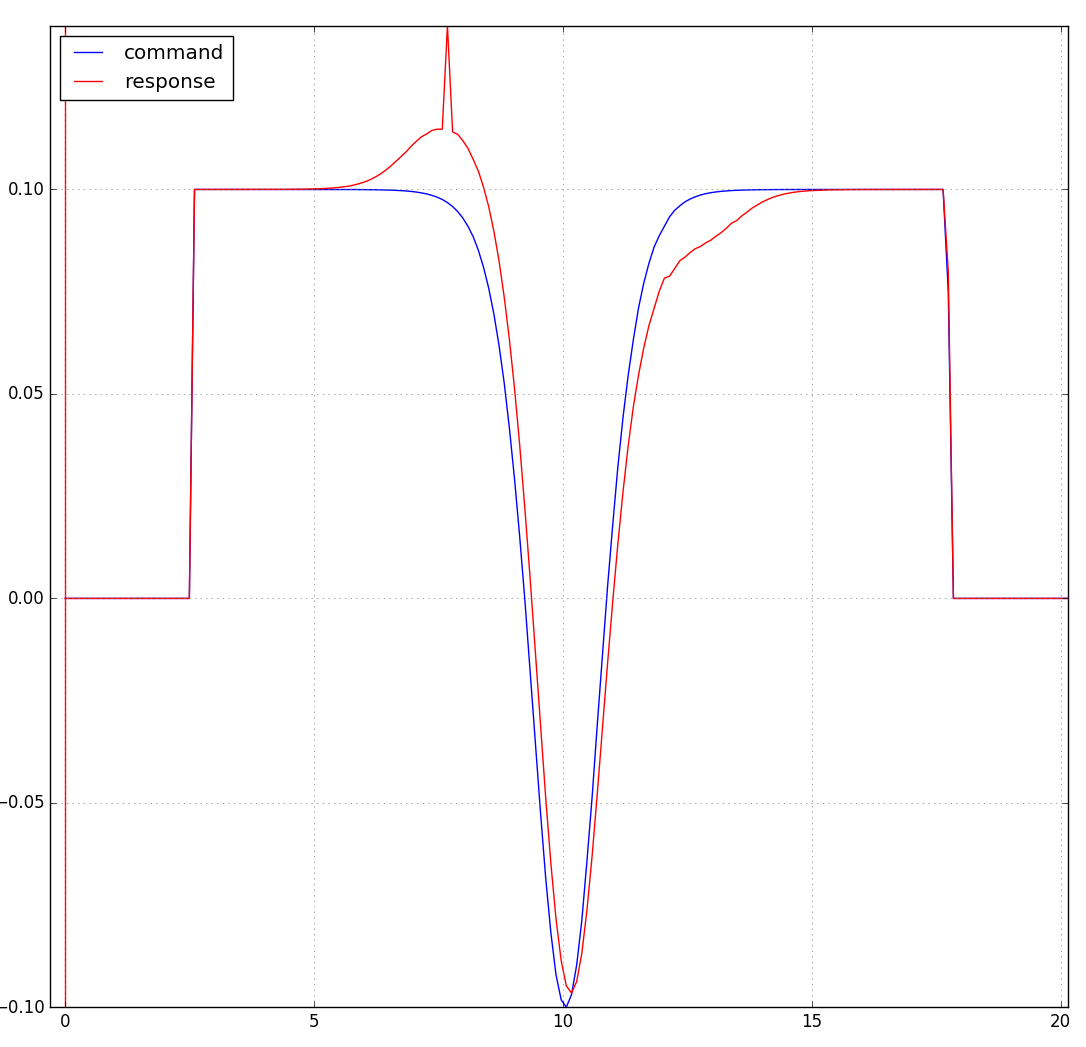
\includegraphics[width=0.6\textwidth]{Figures/360_x.png}
%     \caption{$\dot{x}$}
%     \label{fig:my_label}
% \end{figure}

% \begin{figure}[H]
%     \centering
%     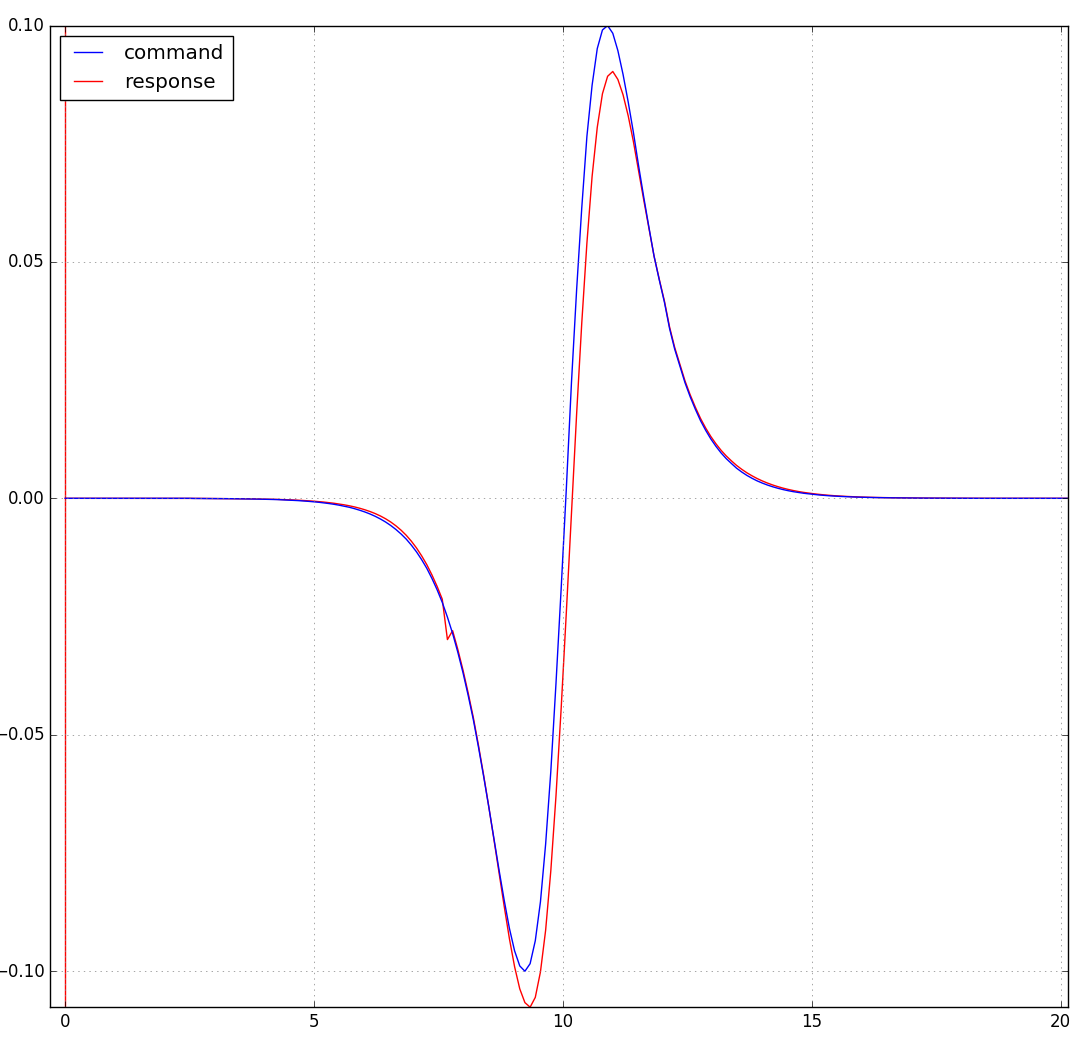
\includegraphics[width=0.7\textwidth]{Figures/360_y.png}
%     \caption{$\dot{y}$}
%     \label{fig:my_label}
% \end{figure}
%%%%%%%%%%%%%%%%%%%%%%%%%%%%%%%%%%%%%%%%%%%%%%%%%%%%%%%%%%%%%%%%%%%%%%%%%%%%%%%%%%%%%%%%%%%%%%%%%%%%%%%%
\subsection{ICR response}
In the ICR space, the ICR response fast with the change of the reference. The sudden change of ICR position is properly handled. The switching between control logic happens at time instance $t=1s$ and $t=16s$ smoothly.
\begin{figure}[!h]
    \centering
    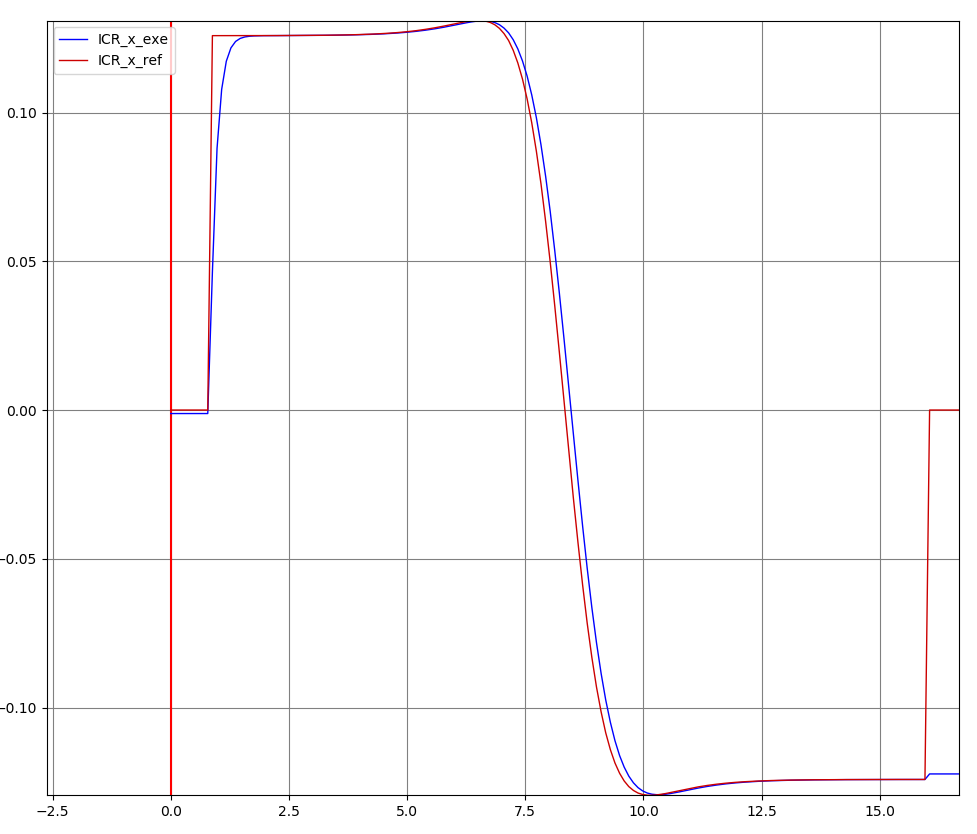
\includegraphics[width=0.75\textwidth]{Figures/360_ICR_x.png}
    \caption{$\Tilde{ICR_x}$}
    \label{fig:360_ICR_x}
\end{figure}

\begin{figure}[!h]
    \centering
    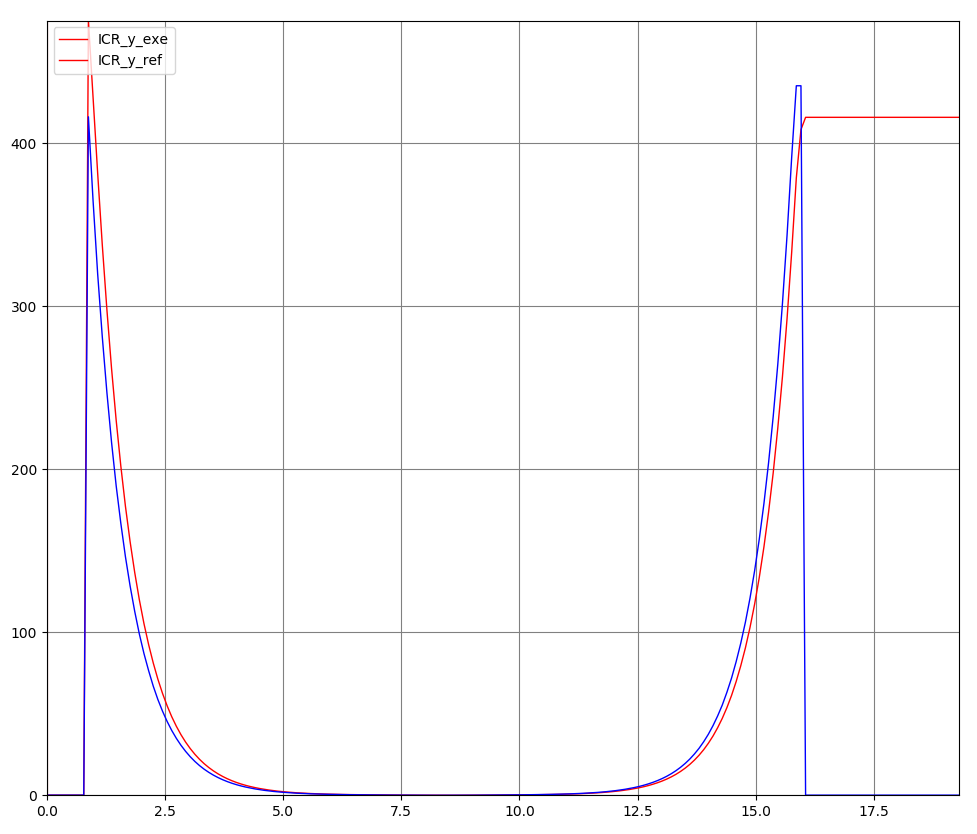
\includegraphics[width=0.75\textwidth]{Figures/360_ICR_y.png}
    \caption{$\Tilde{ICR_y}$}
    \label{fig:360_ICR_y}
\end{figure}

In general the controller response is quite fast and is able to follow the reference joint command we give, this is partly because of the good joint dynamic controller we have on the wheel, which is also a pre-request for our control logic to work. 